\documentclass[12pt]{article}

\usepackage[utf8]{inputenc}
\usepackage[T1]{fontenc}

% clickable links in pdf
\usepackage{hyperref}

% make title variable available
\usepackage{titling}

% create own header footer
\usepackage{fancyhdr}

% images
\usepackage{graphicx}

% grafics powerfull and hard
\usepackage{tikz}

% character spacing to fill line
\usepackage{microtype}

% image placement with [H]
\usepackage{float}

% fancy quotes
\usepackage{epigraph}

% extra symbols
\usepackage{textcomp}

% display code
\usepackage{listings}

% icons
\usepackage{fontawesome}

% set dimmensions of page
\usepackage[footskip=80pt, headheight=15pt]{geometry}

% tables
\usepackage{tabularx}
\usepackage{makecell}

% make code copyable
\lstset{
	upquote=true,
	columns=fullflexible,
	literate={*}{{\char42}}1
	{-}{{\char45}}1
}

\newsavebox{\picbox}

\graphicspath{ {./images/} }

% command for rounded corners
\newcommand{\cutpic}[3]{
	\savebox{\picbox}{\includegraphics[width=#2]{#3}}
	\tikz\node [draw, rounded corners=#1, line width=4pt,
	color=white, minimum width=\wd\picbox,
	minimum height=\ht\picbox, path picture={
		\node at (path picture bounding box.center) {
			\usebox{\picbox}};
	}] {};}


	\newcommand{\apiSpecToblerone}[4]{
	    \begin{table}[H]
	      \begin{tabularx}{\textwidth}{|l|X|}
	        \hline
	        Typ & #1  \\ \hline
	        Name & #2  \\ \hline
	        Content & #3  \\ \hline
	        Beschreibung & #4  \\ \hline
	      \end{tabularx}
	    \end{table}
	}


\begin{document}
	\title{
	\Huge
	\textbf{Globalizer} \\
	\vspace{0.2cm}
	\LARGE
	Detailkonzpet
}

\date{22.11.2018}

\author{
	Koller, Jonas\\
	\texttt{jonas.koller@gmx.ch} \\
	Wolfisberg, Donato \\
	\texttt{donato.wolfisberg@gmail.com}
}

\pagestyle{fancy}
\fancyhf{}
\lhead{BBZW Sursee Rötheli Manfred}
\rhead{Globalizer Detailkonzept}
\lfoot{Jonas Koller \& \\ Donato Wolfisberg}
\cfoot{\thedate}
\rfoot{\thepage}

\renewcommand{\headrulewidth}{1pt}
\renewcommand{\footrulewidth}{1pt}

\renewcommand{\contentsname}{Inhalt}

\begin{titlepage}
  \pagenumbering{gobble}

  \begin{center}
    \vspace*{-2cm}
    \cutpic{0.8cm}{4cm}{logo.jpg}

    \thetitle

    \vspace{2cm}

    \textbf{\theauthor}

    \vspace{1.5cm}

    \thedate
  \end{center}

  \vfill

  \begin{figure}[H]
    \makebox[\linewidth]{
      
\includegraphics[width=1.3\linewidth]{globe.jpg}
    }
    \vspace*{-5cm}
  \end{figure}
\end{titlepage}

\newpage
\pagenumbering{Roman}


	\begin{center}
		\makebox[\textwidth]{
\includegraphics[width=\paperwidth]{nightsky.jpg}}
	\end{center}

	\section{Einleitung}
	Dieses Dokument behandelt das Detailkonzept des Projekts Globalizer. Ziel und Zweck des Dokuments ist es, die fachlichen Anforderungen technisch zu umschreiben, damit diese später implementiert werden können. Zudem soll das Gesamtbild unserer Applikation klar gemacht werden und die Komponenten, sowie der Datenaustausch genau beschrieben werden. Es werden auch all unsere Technologieentscheide vermerkt und begründet. Zusammengefasst soll dieses Dokument also eine klare, wie auch detailierte Übersicht zu den technischen Aspekten unseres Projekts sein.

	\newpage

	\section{Allgemeine Informationen}
	Hier folgt eine kurze Auflistung der Informationen zu diesem Dokument, dem Ent\-wicklungsteam und dem aktuellen Stand.

	\subsection{Projektmitarbeiter}
	\begin{table}[h]
		\begin{tabularx}{\textwidth}{|l|l|X|l|}
			\hline
			\textbf{Name} & \textbf{Vorname}  & \textbf{E-Mail}                & \textbf{Funktion}     \\ \hline
			Koller        & Jonas             & jonas.koller@gmx.ch            & Projektleiter         \\ \hline
			Wolfisberg    & Donato            & donato.wolfisberg@gmail.com    & Entwickler            \\ \hline
			Gian          & Ott               & gian\_ott@sluz.ch              & Prüfer                \\ \hline
			Manuel        & Troxler           & manuel\_troxler@sluz.ch        & Prüfer                \\ \hline
		\end{tabularx}%
	\end{table}

	\subsection{Änderungskontrolle}
	\begin{table}[h]
		\begin{tabularx}{\textwidth}{|l|l|l|X|}
			\hline
			\textbf{Version} & \textbf{Datum} & \textbf{Ausführende Stelle} & \textbf{Bemerkung}                     \\ \hline
			1                & 21.09.2018     & Projektteam                 & \makecell[l]{Erste Version des Dokuments \\ erstellt}  \\
			2                & 23.09.2018     & Projektteam                 & \makecell[l]{Gesamtüberblick erstellt}  \\
			3                & 25.09.2018     & Projektteam                 & \makecell[l]{Zielkatalog erstellt}  \\
			4                & 27.09.2018     & Projektteam                 & \makecell[l]{Abschliessende Arbeiten}  \\
			\hline
		\end{tabularx}
	\end{table}

	\subsection{Prüfung}
	\begin{table}[h]
		\begin{tabularx}{\textwidth}{|l|l|X|}
			\hline
			\textbf{Version} & \textbf{Datum} & \textbf{Ausführende Stelle}     \\ \hline
			4                 & 27.09.2018    & Gian Ott                        \\ \hline
		\end{tabularx}
	\end{table}

	\newpage
	\tableofcontents
	\newpage

	\pagenumbering{arabic}


	\section{Systemkomponenten}
	Das Projekt verwendet einen klassische Client - Server Architektur. Somit ergeben sich bei uns drei Hauptkomponenten. Dies ist das Backend, das Frontend und die Datenbank. Wir werden folgend beschreiben, wie diese genau aufgebaut sind.
	\subsection{Frontend}
	In der Fontend-Komponente soll die Schnittstelle zwischen Endbenutzer und Backend-System implementiert werden. Wir werden dies mit einer Weboberfläche machen. Diese Komponente soll unabhängig vom Backend-System auf einem CDN gehostet werden können. Diese Masnahme verringert die Wartenzeiten des Endnutzers deutlich.
	\subsection{Backend}
	Unser Backend-System soll die Schnittstelle zwischen den Daten und dem Frontend abbilden. Hier werden die rohen Daten von der Datenbank aufbereitet, berechnungen durchgeführt und die Security-Aspekte grösstenteils abgedeckt. Die Authentifizierung, Autorisierung und Überprüfung der übermittelten Daten soll hier stattfinden. Das Backend soll möglichst klein gehalten werden, damit der Wartungsaufwand minimal bleibt. Es soll so gebaut werden, dass es gut skalierbar verwendet werden kann. Aspekte wie Load-Balancing und Upscaling sollen vom Hoster übernommen werden.
	\subsection{Datenbank}
	Die Datenbank bildet den dritten Teil unseres Systems. Hier soll eine InMemory-Datenbank verwendet werden. Diese brauch weniger Leistung und sorgt für zusätzliche Geschwindigkeit beim System. Uns ist bewusst, dass die Datenbank ihren aktuellen Stand bei einem Systemabsturz verlieren kann. Da es sich jedoch um einen flüchtigen Chat handelt, welcher nicht zu 100\% sicher persistiert werden muss, kann eine InMemory-DB verwendet werden.

	\newpage

	\subsection{Zonen-Übersicht}
	Auf der nachfolgenden Grafik kann unsere Architektur im groben ausgelesen werden. Das System ist in die drei "Komponenten-Zonen" unterteilt. Diese sollen wenn möglich unabhängig von den anderen deploybar sein. Dies ermöglicht es uns später auch, unsere Deployment-Zyklen zu vereinfachen. Im Backend-System ist zusätzlich auch der LoadBalancer eingezeichnet, welcher vom Hoster übernommen wird.\newline

	\noindent
	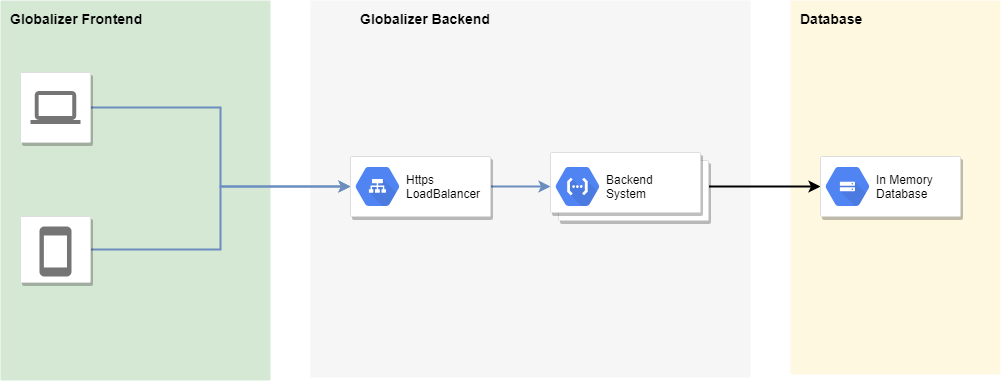
\includegraphics[width=\linewidth]{system-components.png}

	\section{Design-Pattern}
	Da werder unser Backend, noch unser Frontend objektoriertiert ist, können keine Klassendiagramme erstellt werden. OOP-Eigenschaften wie Vererbungen und beziehungen werden bei diesem Projekt auch kaum benutzt. Aus diesem Grund verzichten wir auf diese Diagramme. Wir verwenden anstelle dessen aber ein UML-Aktivitätsdiagramm, um unsere Abläufe zu visualisieren. Wir venwenden in diesem Projekt keine Domain-Driven-Design, Test-Driven-Design oder ähnliches, da unser Projekt zu klein ist, damit dies den Aufwand wert wäre.

	\subsection{Allgemeine Architektur-Pattern}
	Wir wollen die Kommunikation zwischen Frontend und Backend möglich dynamisch und asynchron halten, damit weder das Front- noch das Backend lange Wartenzeiten aufweist oder "einfriert". Da die Kommunikation selbst aufgrund der Technologien nur schwer ganz asynchron umsetzbar ist, verwenden wir das in Angular häufig angewanndte "pseudo Asynchronität". Die Anfragen an sich verlaufen synchron. Angular lässt aber zu, dass das Frontend wärenddessen nicht blockiert wird und arbeitet bis zur Antwort den restlichen Befehlsstack ab und hört auf Events. Im Backend läuft das auch so. Somit blockieren werder das Back- noch das Frontend und der Nutzer hat ein vielfach besseres Erlebnis beim verwenden der Applikation. Sowohl verwenden auch an beiden Orten das "Observer"-Pattern. Dies wird durch Angular und NodeJS unterstützt, in dem wir die "rxjs"-Library verwenden. Durch die einbindung dieser vereinfacht sich das Behandeln von Events und das reaktive Programmieren.

	\subsection{Codestyle und Codequalität}
	Damit unser Projekt auch über lange Zeit verwendbar, Wartbar und Erweiterbar ist, werden wir einige Programmierprinzipien anwenden, welche sicherstellen, dass unser Code langzeitig sauber bleibt. Dies sind folgende:
	\begin{itemize}
		\item \faCode~ Cleancode-Prinzip
		\item \faInstitution~ SOLID-Prinzip
		\item \faUsers~ Pair-Programming-Prinzip
		\item \faGit~ Feature-Branches und Pull-Requests
	\end{itemize}
	Falls einer der Begriffe unbekannt sein sollte, kann eine Erklärung zu diesem im Internet gefunden werden.\newline
	Wir verwenden Github als Versionskontrolle (mehr dazu bei den Technologieentscheiden). Damit wir die oben genannten Prinzipien einhalten, setzen wir \href{https://www.codefactor.io}{Codefactory} ein. Zudem verwenden wir auch \href{https://palantir.github.io/tslint/}{TSLint}, eine Clientseitige Library zur Überprüfung vom Codestyle.\newline
	Desweitern verwenden wir einen Continuous Build System und ein Continuous Testing System, welches aktiviert wird bei einem "Push" ins Github Repository. Dazu auch später mehr.

	\subsection{Architektur Backend}
	Das Backend wird in NodeJS erstellt. Es nutzt Websockets zur Kommunikation mit dem Frontend. Das Websocket-Protokoll ist auf TCP basiert und erlaubt bidirektionale Verbindungen zwischen Server und Client. Das Backend ist offen für neue Verbindungen. Wenn sich ein neuer Benutzer anmeldet, registriert dieser sich beim Backend. Dieses hört danach auf Anfragen des Frontends. Im gegenzug sendet das Backend neue Nachrichten selbst an das Frontend. Durch dieses "Bidirectional Message Pattern" können wir einiges an Bandbreite einsparen, da wir nicht immer wieder Fetch-Anfragen senden müssen um den Client auf dem aktuellen Stand zu behalten. Wir konnten somit das "Fetch"-Antipattern umgehen, da dieses für eine Chat-Applikation ungeeignet ist. In der folgenden Grafik kann ausgelesen werden, wie die der Ablauf bei Anfragen an den Server aussehen.
	\subsubsection{UML Flussdiagramm}
	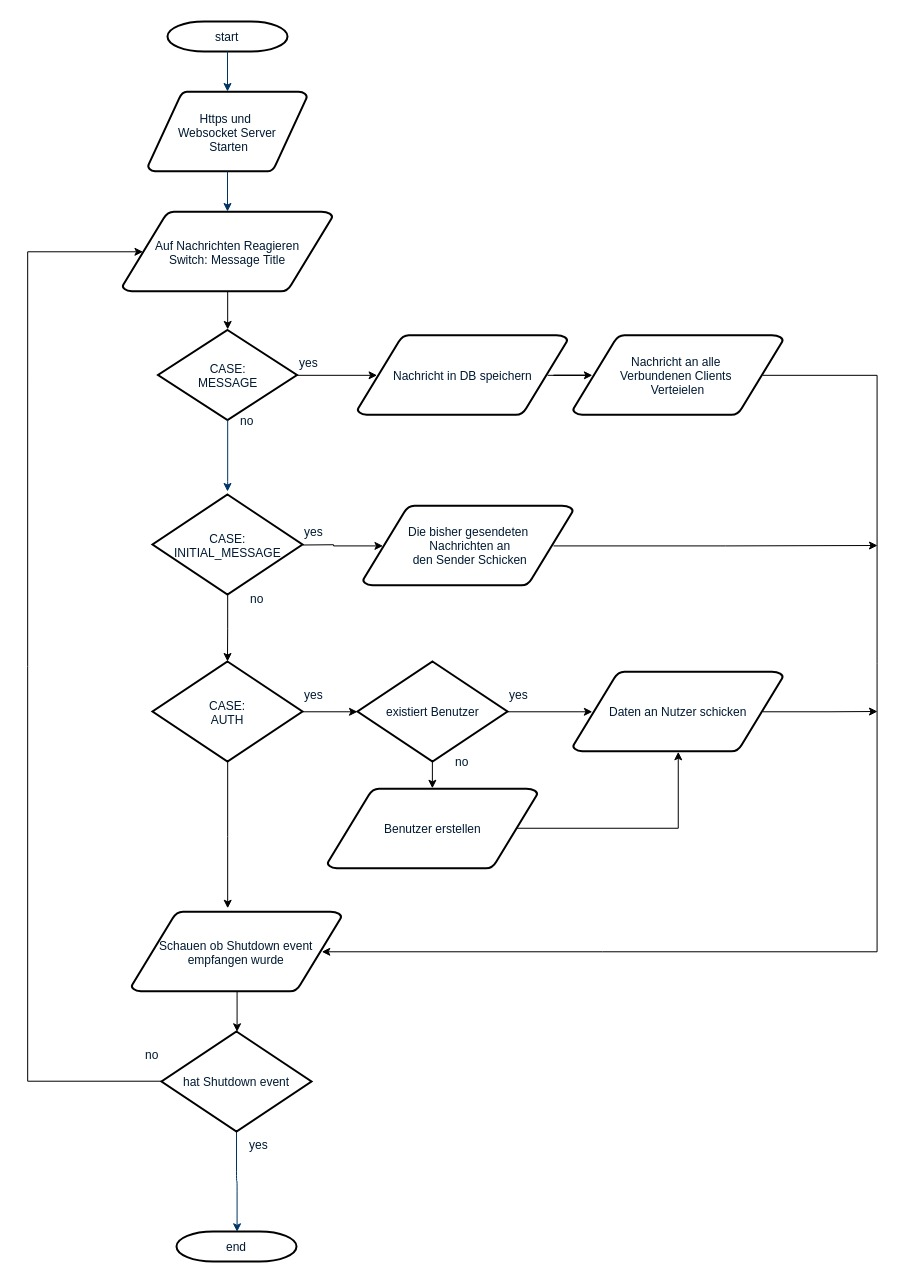
\includegraphics[width=0.9\linewidth]{flow-diagramm-server.jpg}

	\subsection{Architektur Frontend}
	Unser Frontend wird mit Angular (Version 7) implementiert. Wieso genau wir uns für diese Technologie entschieden haben wird später erläutert. Dazu wird das Google Angular Material verwendet, damit wir dank dieser Library nicht alle UI-Komponenten selbst erstellen und designen müssen, sondern auf diese UI-Library zurückgreifen können (diese Library ist ähnlich wie Twitters Bootstrap). Das Frontend sendet auch via Websocket-Protokoll Nachrichten an das Backend.

	\section{Persistenz}
	Unsere Applikation verwendet wie bereits oben beschrieben eine InMemory Datenbank. Diese wird eine NoSQL Datenbank sein (NoSQL im Sinne von kein SQL verwendend und nicht darauf basierend). Sie basiert auf einem JSON-Datenmodel. Dies da wir in JavaScript programmieren werden und die Daten verwenden können, ohne diese zuerst parsen zu müssen. Die InMemory-DB wird durch Vanilla-JavaScript ermöglicht und braucht keine weiter Library. Ein konkretes Datenmodel gibt es nicht aufgrund von dem Fakt, dass wir dynamisch Daten speichen und entfernen und das genaue Datenmodel so entsteht.

	\section{Detailierte Komponenten und Schnittstellen}
	Folgend werden alle Komponenten genau beschrieben und deren Schnittstellen definiert.

	\subsection{Backend}
	Die Backendkomponente bildet das "Hirn" unserer Applikation. Hier werden sowohl alle wichtigen Daten gespeichert (in der InMemory-DB), als auch alle wichtigen Impulse verwendet (Websockets). Ziel des Backends ist es eine möglichst hohe flexibilität und Wartbarkeit mit einer möglichst hohen Performance zu kombinieren. Dies wird durch die sehr junge Backend-Sprache NodeJS ermöglicht.

	\subsection{Funktionale Anforderungen}
	Das Backend ist betroffen von 3 obligatorischen funktionalen Anforderungen. Diese sind:
	\begin{itemize}
		\item \faLock~ USER\_STANDARD\_LOGIN
		\item \faSend~ NACHRICHT\_SENDEN
		\item \faEnvelope~ NACHRICHT\_EMPFANGEN
	\end{itemize}
	Was diese Anforderungen konkret bedeuten kann im Dokument "Anfoderungsspezifikationen" nachgelesen werden. Dort sind diese inklusiv Use-Case-Diagramm dargestellt.

	\subsection{Schnittstellen}
	//TODO: Schnittstellen beschreiben

	\subsection{Presistenz}
	Das Backend übernimmt den Hauptteil der Persistenz der ganzen Applikation. Hier werden alle Nachrichten und Benutzer in die InMemory-DB gespeichert und der Zustand der ganzen Applikation.
	Die Entitäten sehen wie gefolgt aus:\newline
	\noindent
	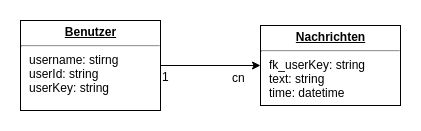
\includegraphics[width=\linewidth]{backend-entity.png}

	\subsection{Frontend}
	Die Frontendkomponente bildet die Schnittstelle zwischen Endbenutzer und System. Hier werden die Daten aus dem Backend grafisch dargestellt. Wichtig an dieser Komponente ist, dass das Aussehen dieser modern und stylisch ist, damit der Nutzer ein tolles Erlebnis auf der Seite hat. Auch Geschwindigkeit ist hier ein wichtiges Thema, weshalb Angular 7 eine sehr gut passende Technologie ist. Die Funktionsweise des Frontends kann aus diesen UML-Diagramm ausgelesen werden.
	\subsubsection{UML Flussdiagramm}
	//TODO: UML Flussdiagramm Frontend (client-flow-diagram.png)

	\subsection{Funktionale Anforderungen}
	Das Frontend ist betroffen von 3 obligatorischen funktionalen Anforderungen. Diese sind:
	\begin{itemize}
		\item \faLock~ USER\_STANDARD\_LOGIN
		\item \faSend~ NACHRICHT\_SENDEN
		\item \faEnvelope~ NACHRICHT\_EMPFANGEN
	\end{itemize}
	Was diese Anforderungen konkret bedeuten kann im Dokument "Anfoderungsspezifikationen" nachgelesen werden. Dort sind diese inklusiv Use-Case-Diagramm dargestellt.

	\subsection{Schnittstellen}
	Die Schnittstelle zwischen Benutzer und Frontend ist rein visuell. Diese soll später so aussehen:

	\subsubsection{Android frame}
	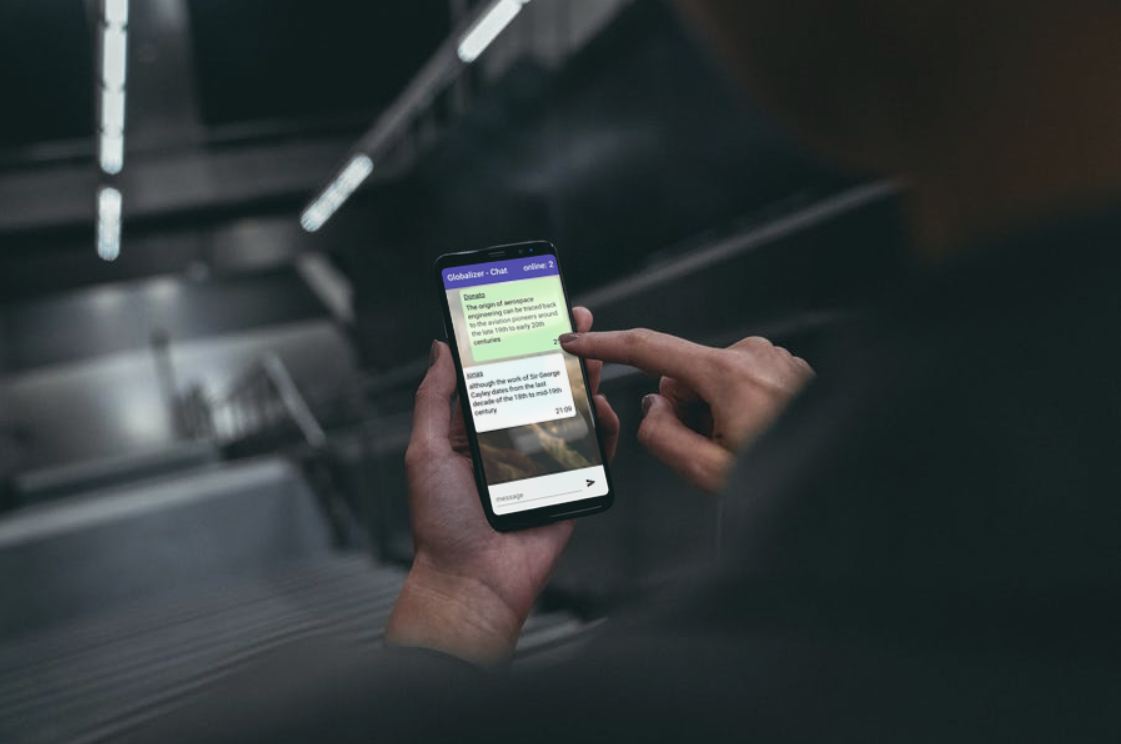
\includegraphics[width=\textwidth]{mock-chat.png}
	\subsubsection{Desktop Chrome Login}
	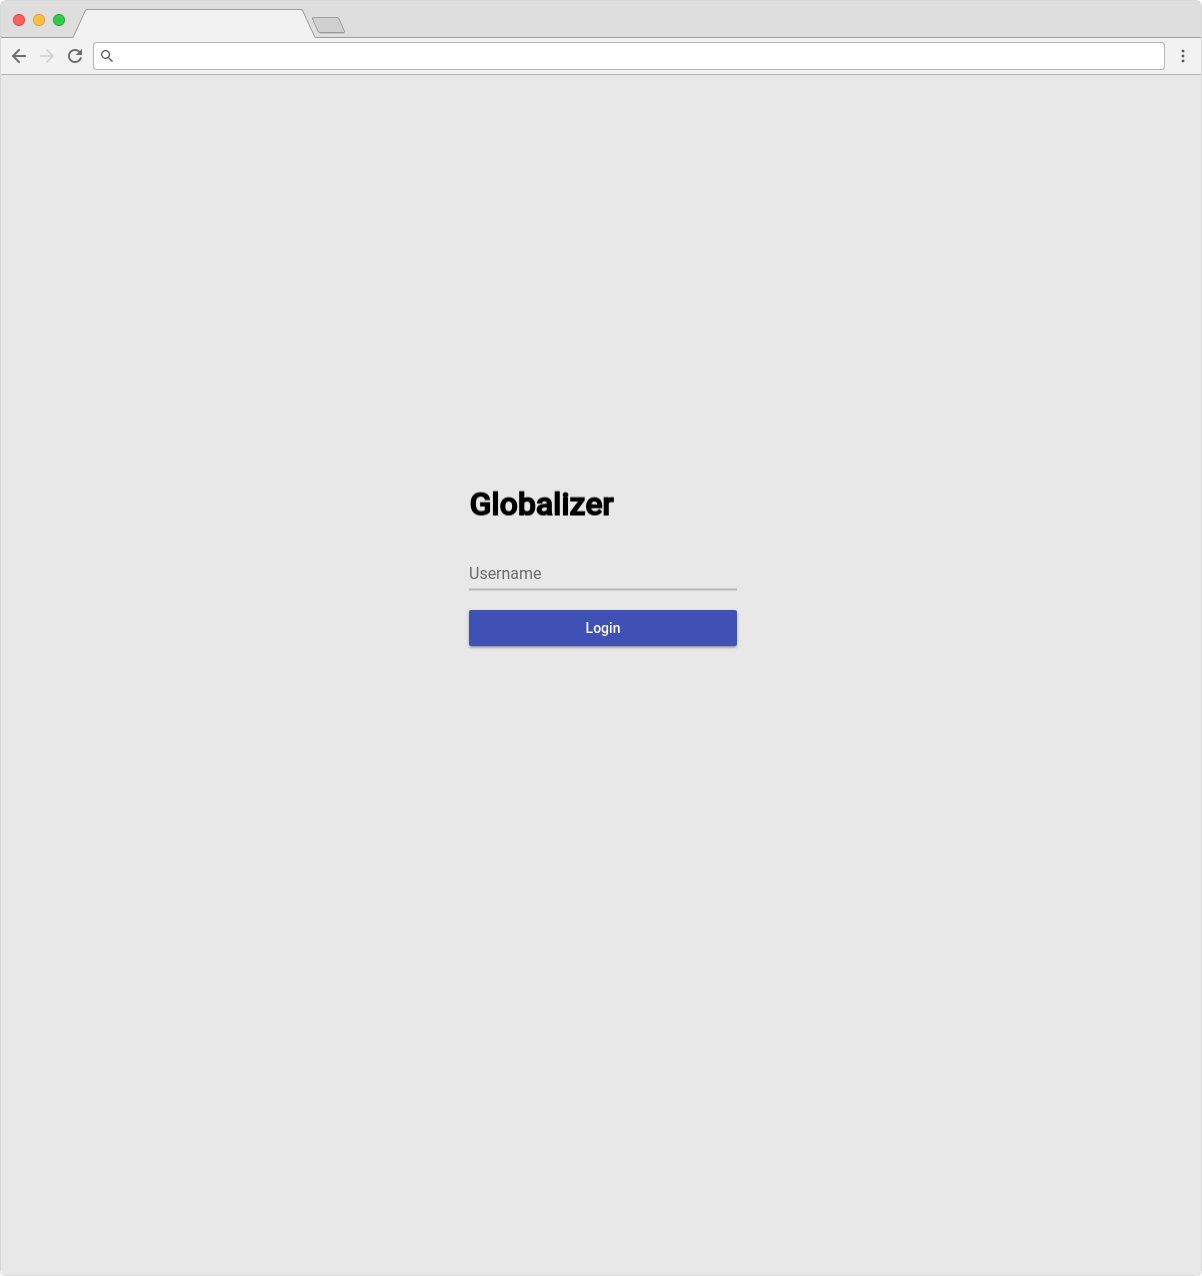
\includegraphics[width=\textwidth]{frame-desktop-login.png}
	\subsubsection{Desktop Chrome Chat}
	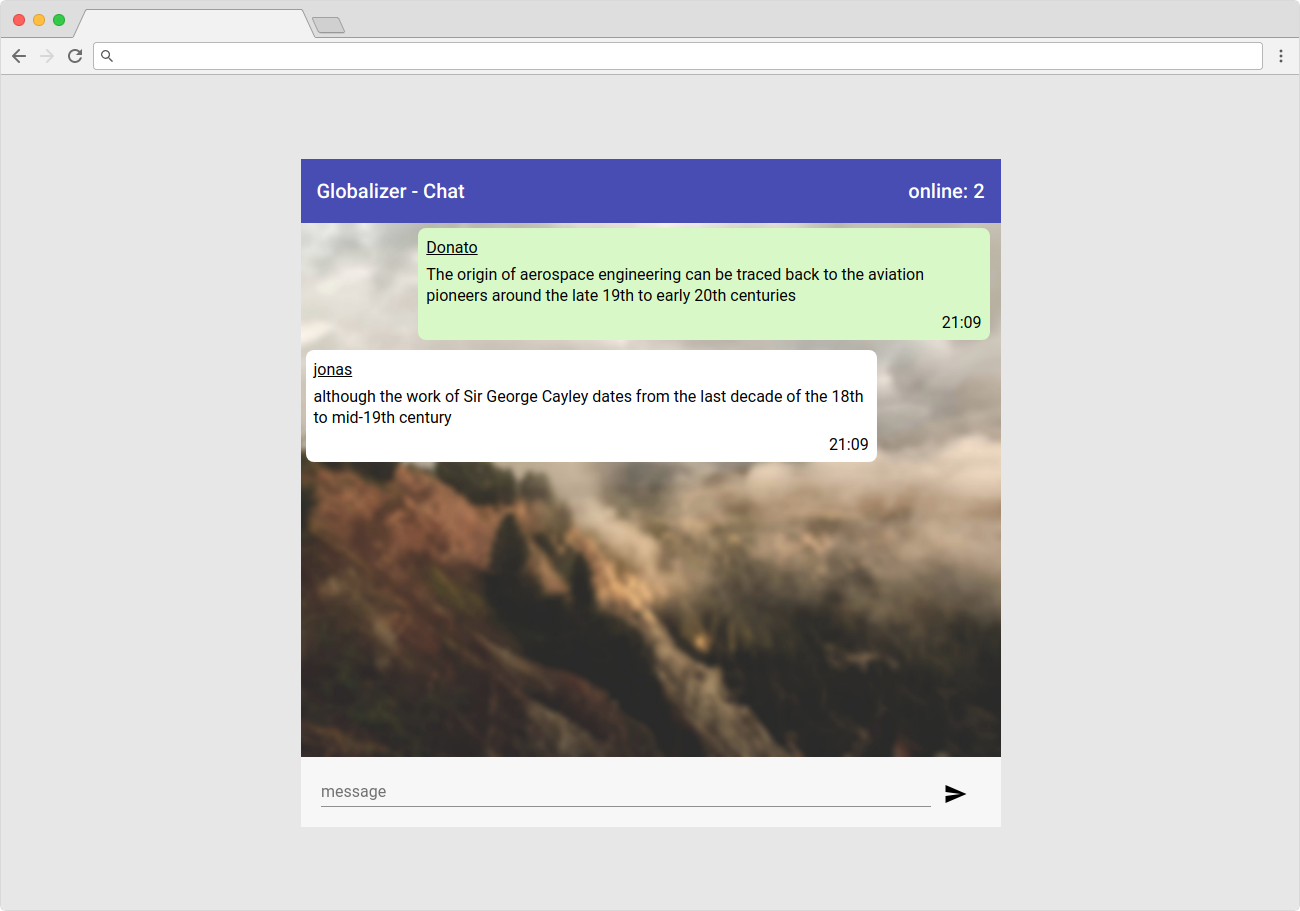
\includegraphics[width=\textwidth]{frame-desktop-chat.png}

	\subsection{Presistenz}
	Das Frontend hat nur einen ganz minimalen Teil an Persistenz. Dazu wird der durch HTML 5 neu eingeführte LocalStorage eingesetzt. Es wird nach dem Login eines Benutzers dessen ID gesichert, damit später ein Sessionlogin durchgeführt werden kann und der Nutzer sich nicht erneut anmelden muss. Da diese Daten aber auf dem Client selbst gespeichert sind, müssen sie mit vorsicht behandelt werden. Der LocalStorage ist ein simpler Key-Value-Store.

	\section{Technologieentscheide}
	In diesem Abschnitt des Dokuments begründen wir, weshalb wir die von uns gewählten Technologien verwenden.

	\subsection{Webclient}
	Wir setzen bei der Schnittstelle zwischen Benutzer und System bewusst auf einen Webclient und nicht auf einen Fat-Client. Dies ermöglicht es uns, dass unsere Applikation erreichbar ist, ohne dass zuerst ein Client heruntergeladen und installiert werden muss. Des weiteren können wir so auch direkt Benutzer mit Smartphones abholen, da wir ein Responsive Design verwenden. Es ergeben sich also einige Vorteile durch die verwendung eines Webclients anstelle des Fat-Clients. Deshablb haben wir uns für diese Variante entschieden.

	\subsection{Angular}
	Unseren Webclient setzen wir mit Angular 7 um. Dies hat zum einen den Grund, dass wir beide schon Erfahrungen mit Angular 7 haben, zum anderen aber auch, da Angular momentan eine der meist genutzten und am besten geeigneten Frontend-Frameworks ist. Für die Version 7 haben wir uns entschieden, da diese eine viel bessere Kompression als die Vorgängerversionen hat. Somit wird die Datenübertragung minimiert und die Geschwindigkeit der Applikation steigt.

	\subsection{NodeJS}
	Wir haben uns für NodeJS entschieden, da es sich hier um eine neue und sehr schnelle Sprache handelt. Wir wollen einen möglichst wartbaren Code. Hier ist Node optimal, da es nur einen minimalen Overhead mit sich bringt. So kann unser Server flach gebaut werden ohne grosse Strukturen um diesen herum zu benötigen. Weitere Punkte die für Node sprechen sind, dass unser Front- und Backend somit die gleiche Sprache verwenden (JavaScript) und die Unterstützung für Websockets hier sehr gross ist, dank einer vielzahl von verfügbaren Libraries.

	\subsection{Github}
	Als Code-Versionskontrolle haben wir uns für Git entschieden, da dies in der heutigen Zeit der Standard ist und wir beide Git bereits kennen und benutzt haben. Als Ablage-Plattform haben wir uns für Github entschieden, da wir auch beide hier bereits Erfahrungen hatten und Github in unserem Fall das kostengünstigste Angebot ist. Da das Projekt die Anfoderung hat, dass es Open Source sein soll, ist Github eine passende Plattform, da auch viele andere grosse Open Source Projekte auf Github setzen.

	\subsection{LaTex}
	Der letzte erwähnenswerte Technologieentscheid ist der des Dokumentationstools. Wir verwenden LaTex, welches geeignet ist um technische und wissenschaftliche Dokumente zu erstellen. Bis jetzt hat noch niemand von uns mit LaTex gearbeitet. Wir haben uns aber für dieses entschieden nach einer intensiven Internetrecherche und einem ersten Testlauf, welchen wir durchgeführt haben.

	\section{Continuous Integration und Testing}
	Wir werden bei unserem Projekt eine Continuous Integration und ein Continuous Deployment eingerichten. Es wird zudem auch ein Continuous Testing geben.

	\subsection{CI mit CircleCI}
	CircleCI ist ein Buildserver, welcher für Continuous Integration genutzt wird. Man kann CircleCI mit Github verbinden und bei jedem Push einen Build "triggern". Somit sieht man direkt, wenn nach einem Push das Projekt nicht mehr gebaut werden kann und Fehler werden sehr frühzeitig erkannt. Dies ermöglicht es uns, dass der Stand welcher auf Github ist immer lauffähig und funktionell ist. CircleCI kann für Open Source Projekte kostenlos genutzt werden. Zu finden unter \href{https://circleci.com/}{https://circleci.com/}.

	\subsection{CT mit Cypress}
	Cypress ist ein weiteres Tool, welches mit Github verbunden werden kann. Es hat zudem auch eine Anbindung an CircleCI. Wir werden Cypress so konfigurieren, dass bei einem Push ein CircleCI-Build "getriggered" wird und das Kompilat aus diesem danach an Cypress übergeben wird. Cypress soll dieses danach laufen lassen und automatisch E2E (End-to-End) Tests laufen lassen, welche uns ein weiteres Werkzeug zur Überprüfung der Integrität unserer Software geben. Cypress ist zu finden unter \href{https://www.cypress.io/}{https://www.cypress.io/}.

#Technologieentscheide
	//TODO: Wieso CI? Und Testing beschreiben //TODO: Testting pipeline bild
	//TODO: Hosting bei Heroku

#testing pipeline

#Deployment
	//TODO: Deploymentdiagramm bild einfügen
\end{document}
